\begin{figure*}[h]
    \centering
    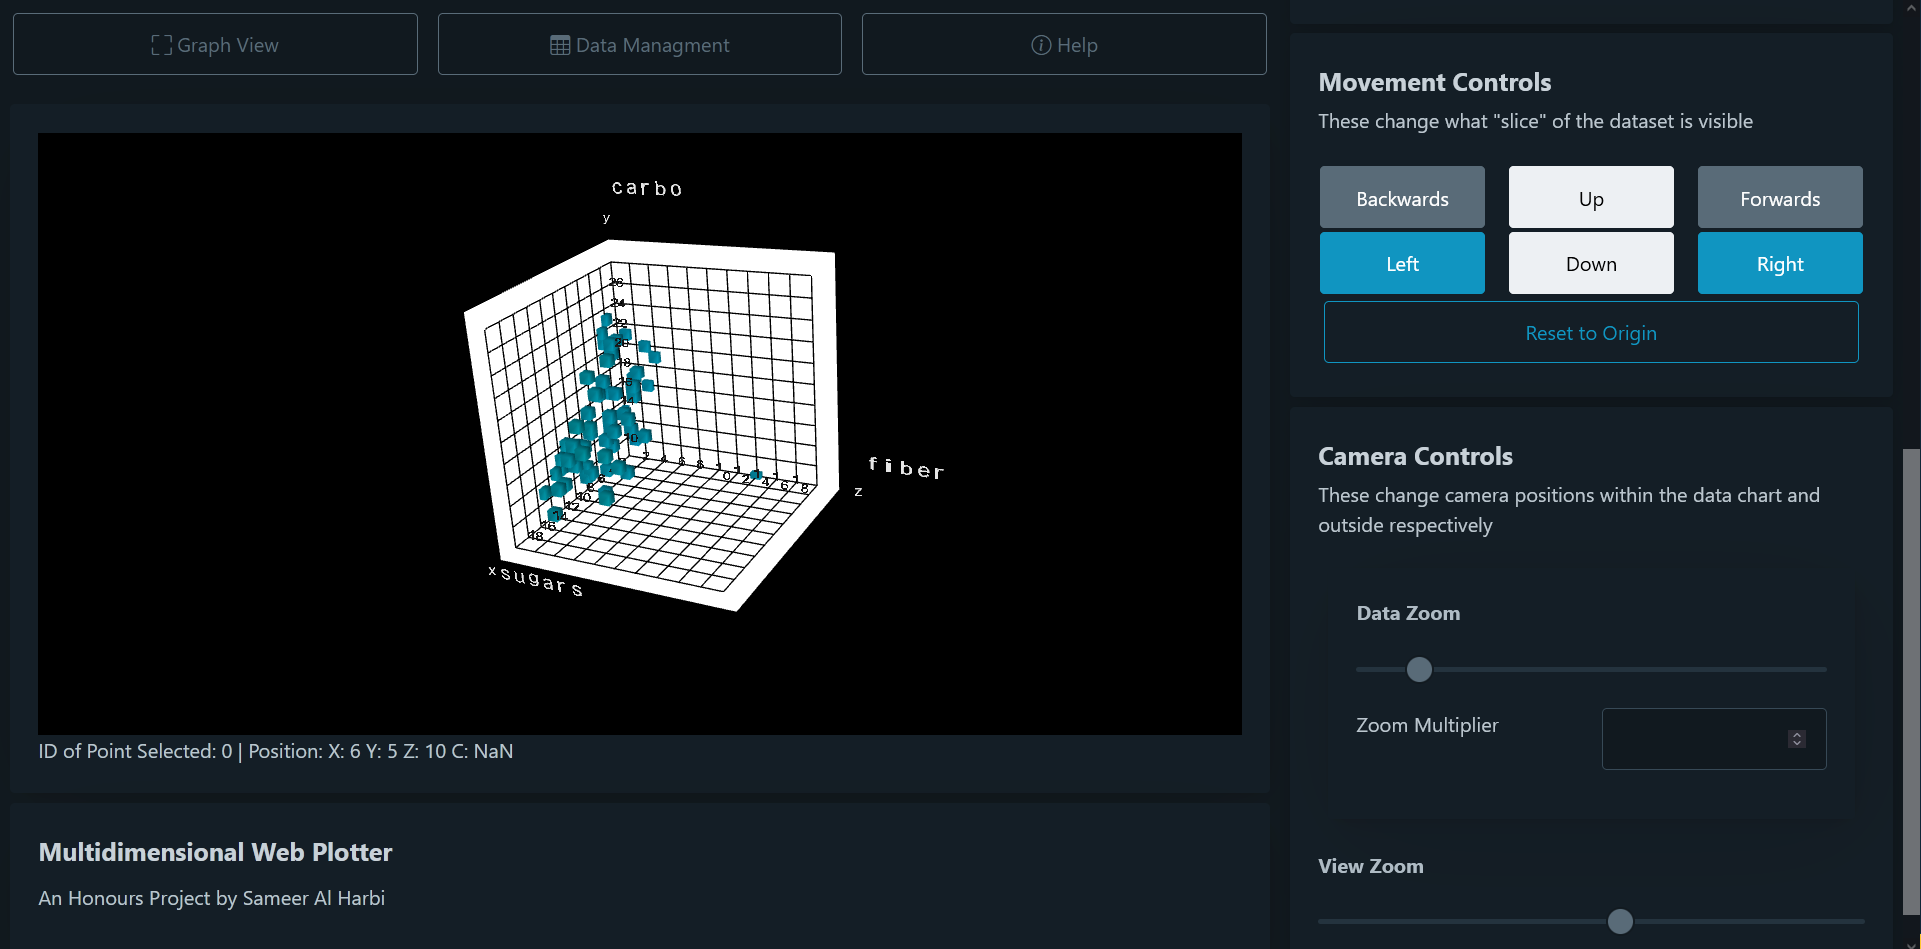
\includegraphics[width=1\textwidth]{author-files/figures/Graph-Fin.PNG}
    \caption{Graph View - Final App Version}
    \label{fig:graphfin}
\end{figure*}
\begin{figure}[h]
    \centering
    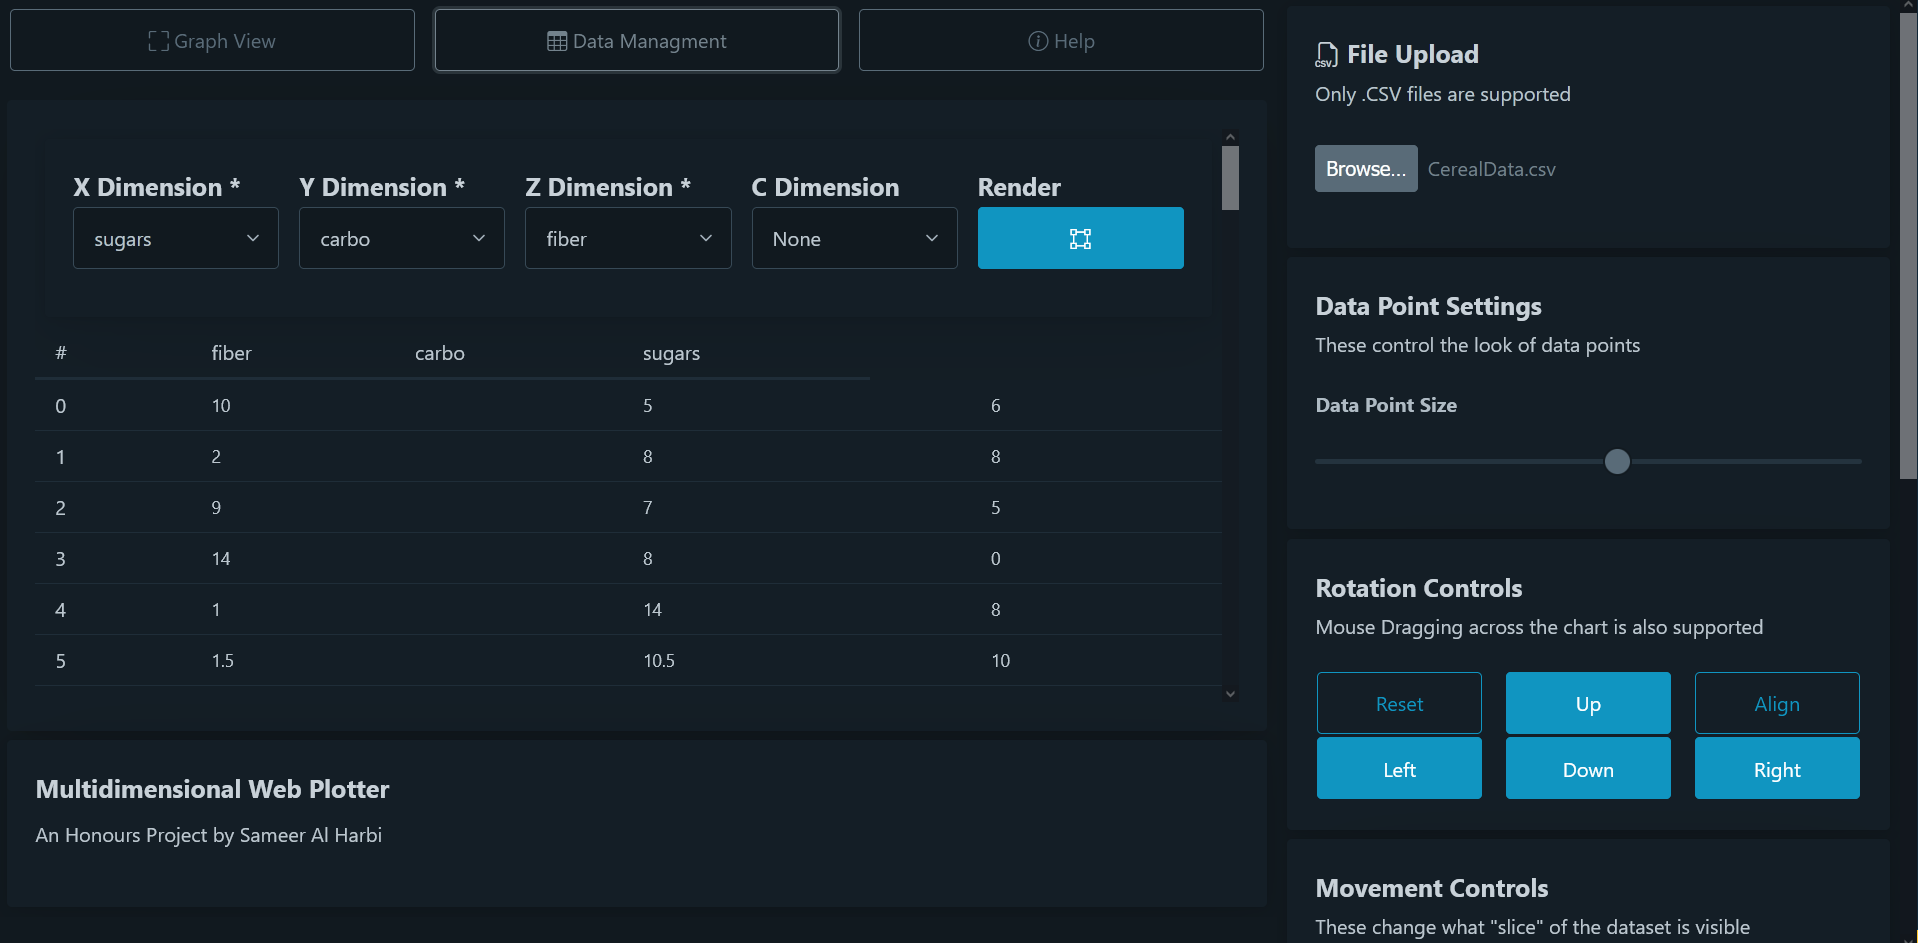
\includegraphics[width=1\columnwidth]{author-files/figures/data-fin.PNG}
    \caption{Data Management View - Final App Version}
    \label{fig:datafin}
\end{figure}
\begin{figure}[h]
    \centering
    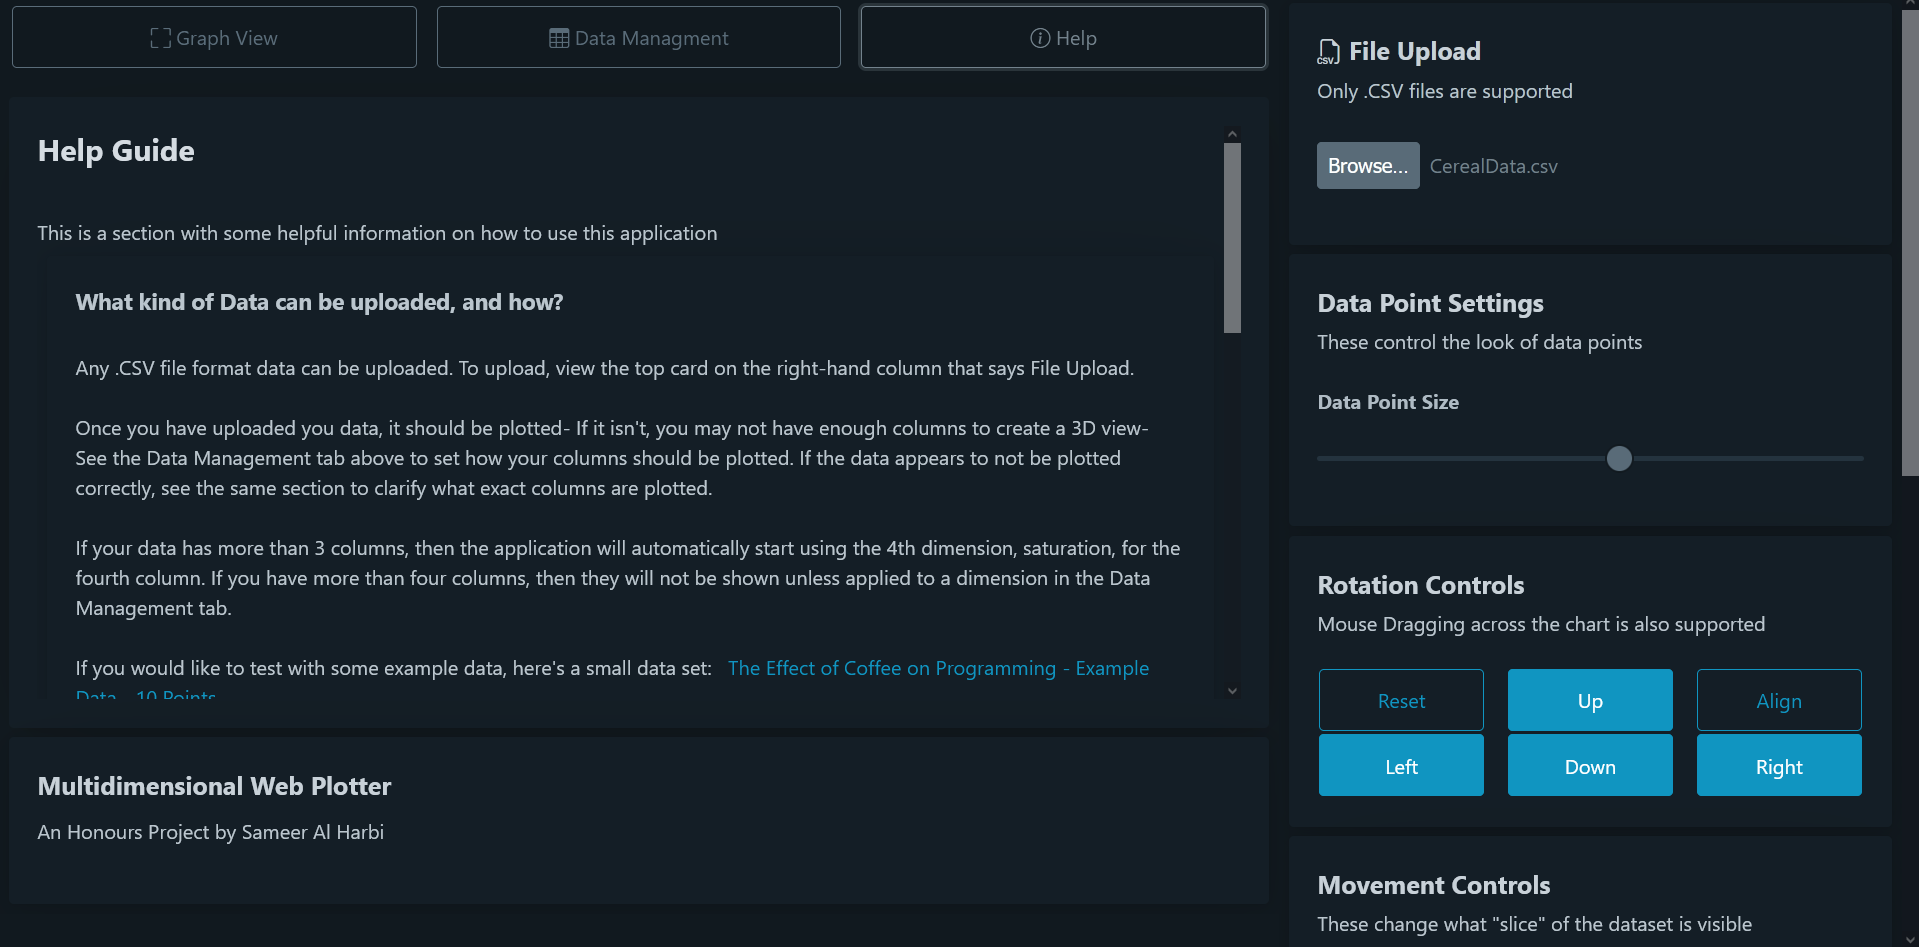
\includegraphics[width=1\columnwidth]{author-files/figures/help-fin.PNG}
    \caption{Help View- Final App Version}
    \label{fig:helpfin}
\end{figure}

\section{Final Product} \label{finprod}
The Application developed is a client-side, web-based plotting application rendering a 3D cube graph showing 10 values on each axis- .CSV data can be uploaded and the user can select which columns to render on which axis's, 3 of which are positional and one modifying the saturation of the plotted point.
Provided user controls include buttons to allow the user to move each axis separately to show a different slice of values, zooming controls to increase or decrease the difference between each axis line, rotation through mouse dragging or button clicking, changing data point sizes, modifying how saturation is applied to labels, selecting points on hover to view the values they represent. The application also allows the user to view the data uploaded in a tabular format.
The application can be accessed on different devices with different screen sizes including mobile devices as long as WebGL and a reasonably modern browser is available. Although highly dependant on device specifications, the application can be reasonably expected to render data with 1,000+ Data points. With Modern laptops found to be capable of rendering at least 40,000 non-decimal Points with acceptable performance.
This functionality is provided by a total of 3 tabs, The Graph Tab (See Figure \ref{fig:graphfin}), The Data Management Tab (See Figure \ref{fig:datafin}), The Help Tab (See Figure \ref{fig:helpfin}).

